\subthesischapter{Generación de reportes estadísticos}
Con el objetivo de obtener estadísticas precisas y eficientes de las rutinas de entrenamiento, se desarrolla el script StatisticsUIController.cs. 
Este tiene la responsabilidad de recuperar los datos almacenados en la base de datos y actualizar los valores pertinentes en 
los gráficos presentados en la figura~\ref{fig: statics-graphs}. Para acceder a detalles específicos del Gráfico 1, el usuario puede 
seleccionar la barra correspondiente al día deseado. En este caso, se mostrarán el valor promedio %como la desviación estándar 
de los datos relacionados con la velocidad y la MCV de las rutinas realizadas, ver figura \ref{fig: statics-graphs} c  .

\begin{figure}[ht]
    \centering
    \subfigure[Gráfico 1]{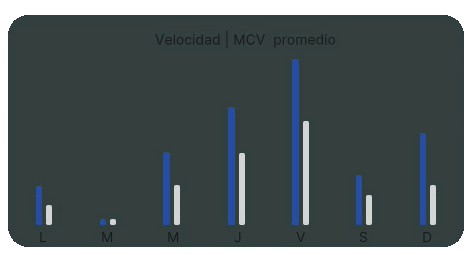
\includegraphics[height=5.2cm, width=0.45\textwidth]{images/ui/ui15-graph1.png}}
    \subfigure[Gráfico 2]{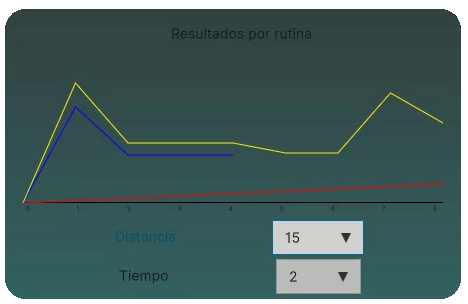
\includegraphics[height=5.1cm, width=0.45\textwidth]{images/ui/ui16-graph2.png}}

    \subfigure[Menú]{
\includegraphics[scale=0.7]{images/ui/ui15-menu.png}}
    \caption{Gráficos estadísticos}
    \label{fig: statics-graphs}
\end{figure}

\subsubthesischapter{Generación de los valores del Gráfico 1}
El primer gráfico (figura \ref{fig: statics-graphs}a) permite visualizar los valores promedio de velocidad y MCV
obtenidos en las rutinas de entrenamiento diarias. Dichos valores se obtuvieron a partir de las ecuaciones \ref{eq: 2} y \ref{eq: 3}.    

\begin{equation}
    V_{i} = \frac{\sum_{j=1}^{k} v_{j}}{k}
    \label{eq: 2}
    \end{equation}
    \begin{equation}
    MCV_{i} = \sum_{c=1}^{4}\frac{\sum_{j=1}^{k} mcv_{c j}}{k}
    \label{eq: 3}
\end{equation}
Donde:
\begin{itemize}
    \item $V_{i} (MCV_{i})$: valor promedio de velocidad(MCV) obtenido el i-esimo día.
    \item $v_{j}(mcv_{cj})$: velocidad(promedio de MCV del canal c) obtenido en la rutina j del i-esimo día. 
    \item $k$: es el número de rutinas ejecutadas el i-esimo día 
\end{itemize}
La representación visual de las estadísticas se logró mediante la manipulación de elementos visuales definidos en el archivo de diseño \textbf{UXML}\footnote{Documento en Unity3D que define la estructura de la interfaz de usuario y las plantillas de interfaz de usuario reutilizables.}. Se crearon contenedores VisualElement para cada día de la semana y se asignaron alturas proporcionales a los resultados promedios obtenidos. Los elementos visuales se actualizan dinámicamente a través del script StatisticsUIController.cs.

\subsubthesischapter{Generación de los valores del Gráfico 2}
El segundo gráfico (figura \ref{fig: statics-graphs}b), permite visualizar los valores de velocidad, distancia y tiempo 
correspondientes a cada rutina de entrenamiento ejecutada. Para ello, se utilizan datos provenientes de las entidades 
de la base de datos, específicamente, de DoEntity y RutineEntity. Estos datos se procesan y se organizan en una representación gráfica compuesta por tres curvas representadas por dichas magnitudes y generadas a partir de la clase SystemCoordinate, donde la coordenada \textbf{x} representa el índice de la rutina y la coordenada \textbf{y} representa la magnitud correspondiente (distancia, tiempo o velocidad). Estas curvas  se visualizan sobre un elemento VisualElement de Unity3D, proporcionando así una representación gráfica clara y comprensible del comportamiento de los datos asociados a cada rutina de entrenamiento ejecutada.
    

\subsubthesischapter{Persistencia de los resultados estadísticos}
En la fase final del juego, se implementó un código crucial para capturar y guardar los resultados obtenidos en la rutina de entrenamiento. Utilizando la clase DateTime de las bibliotecas de c\#, se registra la fecha y la hora exactas del final del juego. Estos datos se almacenaron en una estructura adecuada y se insertaron en la base de datos correspondiente. La clase CibiofibDb facilitó esta operación al proporcionar métodos para añadir datos (addData()) y cerrar la conexión con la base de datos (close()). Este proceso garantizó la persistencia de los resultados en la tabla Do, lo que permite un análisis detallado del entrenamiento en la sesión de estadísticas.